\documentclass[
	12pt,
	a4paper,
	abstract,
	bibliography=totoc,
	chapterprefix,
	headings=openright,
	numbers=endperiod,
	parskip=half,
	twoside,
]{scrreprt}

\usepackage[T1]{fontenc}
\usepackage[utf8]{inputenc}

\usepackage{libertinus}
\usepackage[varqu,scaled=0.95]{inconsolata}
\usepackage{newtxmath}

\usepackage[english]{babel}

% Use less space for the page number
\usepackage[margin=2.5cm,footskip=36pt]{geometry}
\usepackage{graphicx}
\usepackage[htt]{hyphenat}
\usepackage{listings}
\usepackage{microtype}
\usepackage{subcaption}
% Required for listings's upquote
\usepackage{textcomp}
\usepackage{upquote}
\usepackage{xcolor}

\usepackage[hyphens]{url}
\usepackage[hidelinks,pagebackref]{hyperref}
\usepackage[capitalise,noabbrev]{cleveref}

\usepackage[color=ovgu-orange]{todonotes}

\usepackage{lipsum}

\graphicspath{{./figures/}}

\definecolor{ovgu-blue}{HTML}{0068B4}
\definecolor{ovgu-darkgray}{HTML}{606060}
\definecolor{ovgu-lightgray}{HTML}{C0C0C0}
\definecolor{ovgu-orange}{HTML}{F39100}
\definecolor{ovgu-purple}{HTML}{7A003F}
\definecolor{ovgu-red}{HTML}{D13F58}

\lstset{
	basicstyle=\ttfamily,
	commentstyle=\color{ovgu-darkgray},
	keywordstyle=\color{ovgu-blue},
	numberstyle=\ttfamily\color{ovgu-darkgray},
	stringstyle=\color{ovgu-purple},
	rulecolor=\color{ovgu-lightgray},
	frame=single,
	numbers=left,
	language=C,
	breaklines=true,
	breakatwhitespace=true,
	postbreak=\hbox{$\hookrightarrow$ },
	showlines=true,
	showstringspaces=false,
	upquote=true,
	tabsize=4,
	gobble=0,
	captionpos=b,
	abovecaptionskip=\medskipamount,
}

\renewcommand*{\backref}[1]{}
\renewcommand*{\backrefalt}[4]{%
\ifcase #1%
{\color{ovgu-darkgray}(\color{ovgu-red}Not~cited\color{ovgu-darkgray})}%
\or%
{\color{ovgu-darkgray}(Cited~on~page~#2)}%
\else%
{\color{ovgu-darkgray}(Cited~on~pages~#2)}%
\fi%
}

\titlehead{\centering
\includegraphics[width=0.66\textwidth]{OVGU-INF}}

\subject{Bachelor/Master Thesis}
\title{Title}

\author{
Author\\
{\large\href{mailto:christian.grueneberg@st.ovgu.de}{\nolinkurl{christian.grueneberg@st.ovgu.de}}}
}

\date{\today}

\publishers{
First Reviewer:\\
Jun.-Prof. Dr. Michael Kuhn

\medskip

Second Reviewer:\\
Johannes Wünsche

\medskip

Supervisor:\\
Jun.-Prof. Dr. Michael Kuhn
}

\begin{document}

% \frontmatter
\pagenumbering{roman}

\maketitle

\begin{abstract}

% abstract als letztes schreiben, fast kurz die Arbeit zusammen um schnell einen Überblick zu geben
% enthält den wesentlichen Inhalt und die kurz zusammengefasst das Ergebnis der Arbeit
% stellt heraus was der eigene Anteil war/ist
% ca 1 Seite

-> write this last after everything else

\end{abstract}

\tableofcontents

% \mainmatter
\cleardoubleoddpage
\pagenumbering{arabic}

\chapter{Introduction}
\label{cha:introduction}

% Was ist das Problem und warum ist es wichtig.
% stellt heraus warum der Leser sich dafür interessieren sollte
% die Motivation hinter der Arbeit
% beinhaltet auch was ist neu, was habe ich neues zum Thema beigetragen
% was sind die Ergebnisse,
% es wird auch kurz dargestellt wie vorgeganngen wurde
% der Aufbau der Arbeit wird kurz vorgestellt

% possible structure
\section{Overview}

%- general problem for cache replacement\\
%- primary and secondary storage \\
%- memory hierachy\\
%- change due to new trends like cloud storage and increasing cache size\\
%- using of haura storage layer with different cache implementations clock, clock-pro and ml-clock\\
%- tiered storage stack\\
%- describe why using clock based algorithms -> citation in "It's Time to Revisit LRU vs. FIFO"\\

% sollte ich ausfühlricher schreiben vielleicht noch als Diagramm mit rein bringen das cpu Geschwindigkeit sich schneller entwicklet als
% die Geschwindigkeit für Speicherzugriffe 

%Caches are widely used in hardware and software systems today like L3 cache before DRAM, file systems, hard disk drives, databases,
%web servers and many more.
%Caching usually means that a small and fast memory is used before a larger but slower memory.
%However, it can also mean that a memory with different persistency is used, for example an SSD before a hard disk or 
%memory of the same type but in different locations, e.g. in Content Delivery Networks local nodes are used as a cache for distant back-end nodes.
%In all these cases, the goal is to reduce cost, decrease latency, and increase bandwidth.



The table \ref{tab:caching hierarchy} shows a few examples \cite{7569243}.
Caching is used at different level of the memory hierarchy with various cache block sizes, in software or with hardware support and for memory with different latencies.
Therefore many different cache replacement algorithms were proposed for different use cases.

% could describe why clock-based algorithm and not list based were considered.


\section{Contribution}
% check if contribution or contributions is right
- new is direct comparison of clock based cache replacement algorithms\\

\section{Outline}
- description of the structure of the following work\\

% 5-10%, ca. 2-5 Seiten 

\chapter{Background}
\label{cha:background}

% darstellen der nötigen Informationen und Arbeiten um die weitere Arbeit verstehen zu können
% nicht zu weit ausschweifen
% 10-20%, ca. 4-10 Seiten

- next chapter gives a short overview of topics necessary to understand the following work\\

\section{$B^{\epsilon}$-tree}

% own section for $B^{\epsilon}$-tree
%The $B^{\epsilon}$-tree is a write-optimized version of the B-tree, which are widely used for filesystems or databases, with better performance for insert, range queries and key-value updates \cite{bender2015introduction}.
%Unlike the B-tree, the $B^{\epsilon}$-tree has a buffer for each node, where changes to the subtree associated with the node are stored and
%only when the buffer overflows, the changes are written to the nodes of the subtree, which reduces the number of write operations and the data fragmantation.

The idee for the $B^{\epsilon}$-tree was introduced by \cite{brodal2003lower} in a study of the tradeoff between insertions and queries for comparison-based external memory dictionaries.

The basis for $B^{\epsilon}$-trees is the B-tree, which has good performance on queries but suffers from poor performance on small writes, as shown in \cite{bender2015introduction}, 
because the entire node must be updated for each small write.
However, if you reduce the node size to optimize small writes, sequential read performance suffers because many smaller nodes have to be fetched from disk instead of fewer but larger ones.

To optimize for both cases, the $B^{\epsilon}$-tree adds a buffer to each internal node of size $B - B^{\epsilon} $ with $ 0 \leq \epsilon < 1$ as shown in figure \ref{fig:structure B-epsilon-tree}.

\begin{figure}[ht]
	\centering
	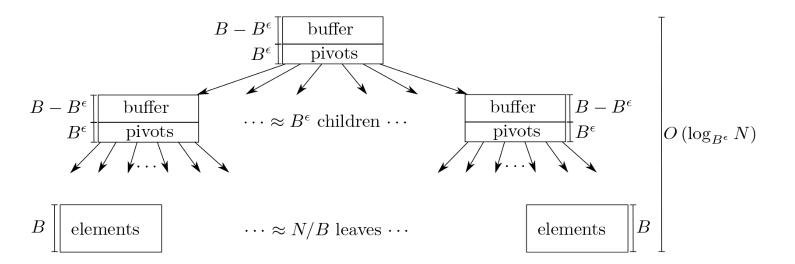
\includegraphics[scale=0.6]{B-epsilon_structure.png}
	\caption{Structure $B^{\epsilon}$-tree from \cite{bender2015introduction}}
		\label{fig:structure B-epsilon-tree}
\end{figure}

As new data is inserted into the $B^{\epsilon}$-tree, the data is written to the buffer of the root node as "insert message".
Only when the root node's buffer is full, a batch of messages is flushed down the tree, preferably to the node with the most pending messages. 
If a node needs to be split, the buffer is also split between the new nodes.
When the insert message arrives at a leaf node, the data is added to the leaf.

This behaviour leads to the better insertion performance then B-trees, because insertion always happens at the root, no searching for the right insertion location necessary and 
the actual write of data happens delayed in batches only when enough changes are accumulated in a buffer.
On deletion a "tombestone message" will be insert into the tree and will be flushed down the tree to a leaf, like an insertion message.

For queries, in the $B^{\epsilon}$-tree, we also need to check the buffer on the way to the leaf nodes to see if there are any relevant messages.
These messages must be processed, but this does not mean that these messages are flushed down immediately, this can happen later.

So the $B^{\epsilon}$-trees achieves similar asymptotic I/O cost for queries but is better for insertions compared to B-trees.

\section{Haura}
%- introduce haura storage stack and explain structure\\
%- short explaination B-epsilon-tree\\
%- task of the cache\\

\todo[inline]{check definition for haura with Johannes}

Haura is a research storage stack written primarily in Rust.
Unlike traditional file systems, haura runs in user space rather than kernel space.
Also, haura uses a key-value and object interface rather than the usual POSIX interface.
It can be used either directly by an application, in which case haura runs in the process context of the application, or
use JULEA as a wrapper for haura.
JULEA then runs the haura instance detached from the user applications, which means that the user application can be terminated or new applications can be created as long as JULEA is running, resulting in more flexibility compared to direct use.

\todo[inline]{insert schemes from haura docu for better understanding}
\todo[inline]{insert link to haura docu as source}
\todo[inline]{epsilon is written diffrently then in original paper}

The development of Haura started to compare $B^{\epsilon}$-tree to ZFS and ext4 filesystem \cite{wiedemann2018modern}, where the haura stack
achieved an improved write performance especially for small random write workloads and better sequential throughput.
Then Haura would be extended by \cite{hoppner2021design} to support multiple stoarge levels
The work of \cite{hoppner2021design} extended Haura with an object storage interface and the support of multiple storage levels while preserving the benefits of the $B^{\epsilon}$-tree.

As pointed out by \cite{wunsche2022data} the advantage of Haura is that all levels which a relevant to implement and optimize a storage stack a combined in a single codebase, so that it is easy change subsystems and test different approaches.
Haura is structured in layers as shown in figure \ref{fig:structure haura}.

\begin{figure}[ht]
	\centering
	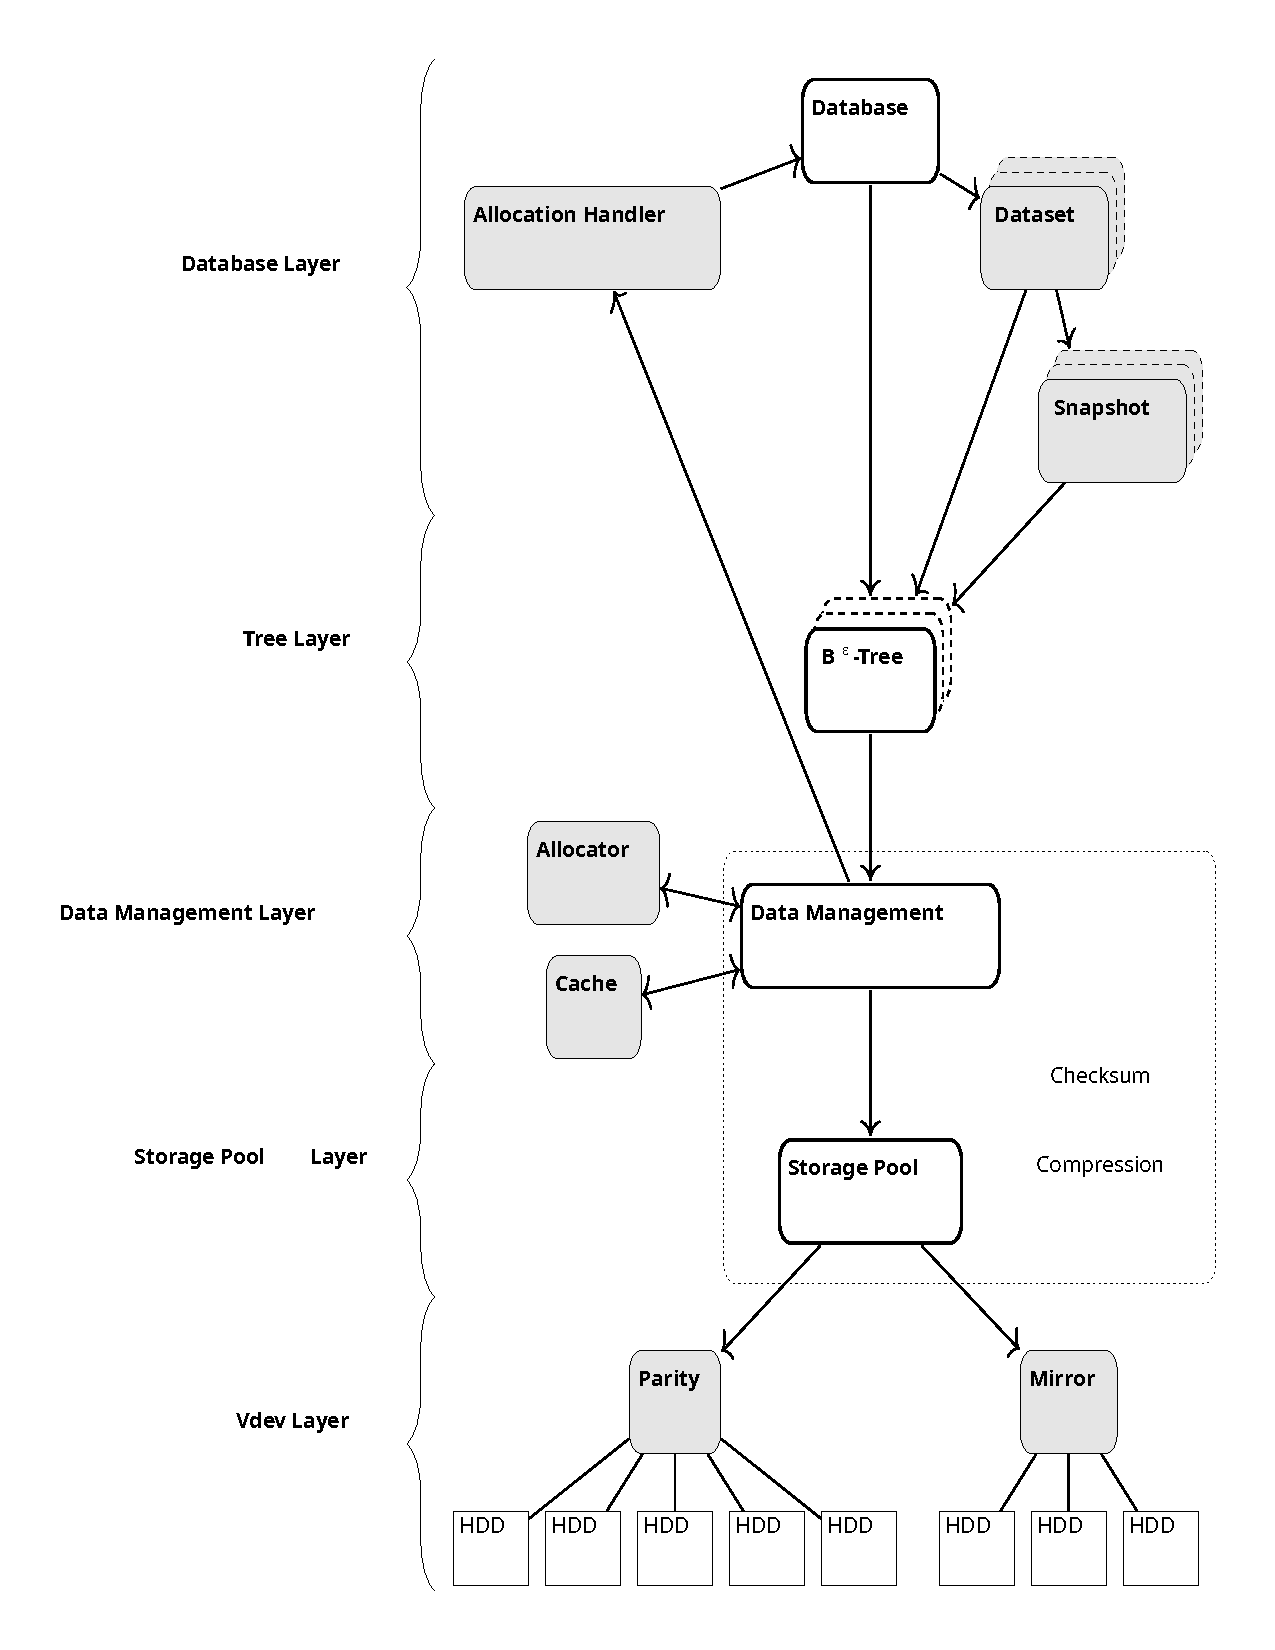
\includegraphics[scale=0.4]{overview_haura_level.pdf}
	\caption{Structure haura, from \cite{wiedemann2018modern}}
		\label{fig:structure haura}
\end{figure}
\todo[inline]{check were I have to put the source for the figure, in text or under the figure}


At the top is the \emph{Database Layer} which manages multiple datasets and snapshots. Each dataset provide a key-value interface, snapshots only read-only key-value interface. Also for each dataset exists an own $B^{\epsilon}$-tree and additonally a root tree which saves the allocation bitmaps and metadata.

The next layer, the \emph{Tree Layer} manages the $B^{\epsilon}$-trees.
The \emph{database layer} sends messages to the $B^{\epsilon}$ trees consisting of key-value or key-message pairs that the $B^{\epsilon}$ trees process. A message for key-message pair can contain arbitrary data or apply arbitrary code on data.
Key-value pairs are stored in leave nodes and key-message nodes are stored in inner nodes of the tree.
Each node is an object for the \emph{Data Management Layer} and is tracked individually.

The \emph{Data Management Layer} manages objects for the \emph{Tree Layer} and \emph{database layer} which means cache objects in memory, 
track modifications to objects and write-back modified objects.
Main part of the \emph{Data Management Layer} is the Data Management Unit (DMU).
The DMU is shared by all trees and ensures that no irregular state can be reached.
It takes care of critical disk management such as block allocation.
In addition, the DMU manages the cache, which is the main topic of this work.

The \emph{Storage Pool Layer} is an abstraction over the used storage hardware.
Furthermore the storage is dvided in to tiers from \emph{Fastest}, \emph{Fast}, \emph{Slow} to \emph{Slowest}.
The user can decide how the used hardware falls into these tiers. Also, not all tiers need to be used.

The last layer, the \emph{Vdev Layer} is responsible for actually reading and writing data from the disks.
Single disk, multiple disks or RAID-like configurations can be used.

\section{Caching}
\subsection{Overview}
There is a large gap between cpu frequency, which is much faster, and  latency and bandwidth of memory.
To reduce the gap and also reduce the cost of a system, memory is arranged in a hierarchy.
Fast but expensive Memory at the top and descending slower but cheaper Memory.
The goal is to find balance between performance, latency and bandwidth on one side and cost on the other side.

\todo[inline]{insert image for memory hierarchy, use it to explain}

% I need to formulate this better
Caching refers to a fast and often smaller primary memory in front of a larger but slower secondary memory, in which the most recently or most frequently used data from the secondary memory is stored for faster access.
It can also mean that data from a remote memory is stored in local memory for faster access, such as a web cache.
The idea of caching is based on the assumption locality.
Mainly temporal locality, when a datum is access it will likely be  accessed again and spatial locality, which means that when a datum is access it is likely that a datum nearby will be accessed in the near future.
For spatial locality usually a block, also called cache line, of many data will be placed and evicted in the cache.
The size of a cache line differs based on size of the cache.

Due to the use of a memory hierarchy, caching is used in several places, as shown in table \ref{tab:caching hierarchy} and can either be handle in hardware like the L1 and L2 cache of a cpu-core, in software like a web cache or a combination of both.

A cache hit occurs when the cache contains the requested data. If the cache is then also full and the requested entry cannot simply be added to the cache, a cache block must be found that is to be removed for the new entry.
To find this victim entry there are several different policies.

\subsection{Optimal Cache Replacement Policy}
The optimal policy, also called Belady's policy, would be to always evict the entry that will not be needed for the longest time.
But this is in general impossible to predict and only known after experimentation and can then be used to compare the optimal solution to other caching algorithm.
Since the optimal solution cannot be obtained, different approximations are used.
The three most used are First-in-First-out(FIFO), Least-Recently-Used(LRU) and Least-Frequently-Used(LFU).

\subsection{FIFO}
The simplest strategy is FIFO, which is not a true approximation of the Bélády's algorithm.
With this strategy, the entry that has been in the cache the longest is always evicted first.
This is very easy to implement and also has the advantage of not having to maintain additional data for each entry or a complex data structure. A simple linked list is sufficient.
However, the serious disadvantage is that FIFO suffers from the Bélády's anomaly, which means that a larger cache size can lead to a higher cache miss rate. LRU and LFU do not suffer from this anomaly.
Although FIFO is simple and easy to implement and is better suited for multi threading because no lock contention occurs when maintaining an ordered linked list during cache hits, it has worse hit rate compared to LRU and LFU.

%Both, LRU and LFU are based on a ordered linked list, like FIFO.
%LRU ordered based on the recency of the last access and LFU based on the access frequency.
%So both have to save extra data for every entry and also have to maintain a ordered linked list which FIFO doesn't.
%At the cost of more effort, a better hit rate is achieved.
%Both LRU and LFU are to expensive and only approximations are used.
% better describe both separately  

\subsection{Least Recently Used}
Another often used cache replacement policy is Least-Recently-Used(LRU).
LRU is an approximation of the optimal Bélády's algorithm.
But in contrast to Bélády's algorithm LRU is an online algorithm and has to select the eviction entry only based on past information.
All cache entries are sorted based on there recency in a linked list.
Each time an entry needs to be evicted, the entry that has not been used for the longest time is evicted.
One problem is that an ordered list is used, i.e. after each cache hit the order in the list may have to be changed, which takes extra time and is done behind a lock for multi threading applications to prevent inconsistencies.
Also to use the last actual access time is to expensive and only approximations are used.
LRU works reasonably well in application with strong locality, CPU caches for example.
On the other hand for applications in which several entries are accesses repeatedly, like looping over an array, LRU is not the best policy, due to neglect of frequency information.
Furthermore applications with repetitive access patterns larger then the cache size are not handled well and lead to higher miss ratio.
Usually LRU has better hit ratio then FIFO \cite{van1992lru}.
Cache replacement algorithms based on LRU are widely used for example ... .
% sources: "An experimental comparison of cache algorithms"
% "LPR: Learning-based Page Replacement Scheme for Scientific Applications"

\subsection{Least Frequently Used}
The last important cache replacement strategy is Least-Frequently-Used (LFU).
The idea behind this is that a cache entry that has been used frequently in the past will also be used in the future.
When a cache miss occurs, the least frequently accessed entry will be evicted.
In case more then one entry have the same access count we have to use recency or decide randomly which entry has to be evicted.
Also the entries are ordered in a single linked list and each entry has an counter which increased for each access.
So we have the same problem as with LRU. We have to keep an ordered list.
Like LRU often only an approximation is used because to track all information is to expensive.
Instead of an Frequency counter for all possible entries only the entries actually in cache have a counter.
Secondly often only a few bits are used as counter so the number of accesses is which can be tracked is limited. 
The advantage of LFU is that entries with a low or 0 access count are removed relatively quickly, while entries with frequent access remain in the cache.
This is the reason why LFU works better than LRU in scanning scenarios.
One problem is that in cases an entry with high access count which is then not or seldom access, is hard to evict even so it is rarely used.
Also LFU don't use or factor in recent access pattern like LRU.
To mitigate this case, aging is used, i.e. after a specified time the counter is reset or decreased.
But this is extra work.
% sources: "An experimental comparison of cache algorithms"
% "LPR: Learning-based Page Replacement Scheme for Scientific Applications"
% wikipedia

\subsection{Improved cache Replacement Policies}

LRU is simple, uses very limited information and works good in cases of strong locality.
Also LRU is the most used or the most policies are based on LRU.
But the downside is scan and loop cases in which LFU performs better.
Researcher tried to improve cache replacement with different ideas.

First explicitly provided hints given by the user.
This seem like a good idea but this is highly application specific and also depends on the hardware.
So for every case someone has to program this into the code of an application.
This is way to much work.
Proposed by \cite{cao1994application} and \cite{patterson1995informed}
% more informatin in LIRS paper

First improvement strategy is through user or application given hints.
This idea was proposed by \cite{cao1994application} and \cite{patterson1995informed}.
It can achieve better performance then LRU but the user must know the underlying access pattern of his application to give good guidance.
It is better to achieve improvement without explicit hints because i
I/O pattern not always known upfront.
Could also be hardware dependent and change from system to system.

Second approach is to use deeper history information because LRU only uses the last reference and not more.
One example is LRU-K proposed by \cite{o1993lru},
which uses the k-last references, mostly k=2 is the best choice.
This is simple and easy to implement but it can quickly remove new and seldom used entries but recently and often used are harder to evict.
For application with significant differences between access of entries this works well but on relatively equal distributed accesses it doesn't perform as well.
Also we still have the cost for maintaining a priority queue.
Another approach for  deeper history information is LRFU \cite{lee2001lrfu}. 
It tracks frequency and recency for each entry and uses a weighting factor $\lambda$ do decide which is more important.
But $\lambda$ is crucial for performance and highly dependent on system and application,
so not really generally applicable.
Another example is 2Q  algorithm by \cite{shasha19942q} which uses multiple queues.
An A1in FIFO queue for new entries, Aout for entries recently evicted, so not resident in memory only meta information and Am as the main buffer for frequently accessed entries.
The problem is again that the user have to set parameters for the A1in, A1out and Am and Thresholds when an entry will be promoted to Am and for switch from A1in to A1out.

The third approach is to detect and adapt to access patterns.
One example is Low Inter-reference Recency Set (LIRS) \cite{10.1145/511399.511340} which uses a queue for cold entries with high inter-reference recency and a queue for hot entries with low inter-reference recency.
Only cold resident entries will be evicted the chance to evict a hot entries is low, need to change to cold entry first.
LIRS is the basis for clock-pro.
We again have the problem that we have to set parameters which are application dependent queue sizes but it is somewhat adaptable clock-pro even more.

Another example is Adaptive Replacement Cache (ARC) \cite{270366}.
ARC shares some similarities with 2Q, it also uses 2 queues $L_1$ for entries entries who are referenced only once in the recent past and $L_2$ for entries accessed at least twice in the recent past.
So  $L_1$ measures recency and $L_2$ the frequency.
To achieve adaptability the sizes of both queues is not fixed but depends on the workload and can change over time.
ARC can outperform LRU and LFU on many real-world traces.

A very recent trend is to incorporate ML-techniques to learn the underlying access pattern.
One example is Fuzzy Page Replacement Algorithm by \cite{akbari2020page}
which used Fuzzy c-means algorithm to find cluster in set of all cache entries an base the decision for eviction on the cluster.
Another example is Learning-based Page Replacement (LPR) by \cite{kim2022lpr} which uses 
uses LRU and MRU and learn the weighting factor between the two policies through online through reinforcement learning.
ML-clock also falls into this category.


\begin{table}[ht]
	\centering
	\begin{tabular}{|l|l|l|l|l|}
		\hline
		\textbf{Cache Type} & \textbf{What Cached} & \textbf{Where Cached} & \textbf{Latency} & \textbf{Managed By}\\
		 &  &  & \textbf{in cycles} &  \\
		\hline
		\hline
		Registers & 4-byte word & CPU registers & 0 & Compiler \\
		\hline
		TLB & Address translation & On-Chip TLB & 0 & Hardware \\
		\hline
		L1 cache & 32-byte block & On-Chip L1 & 1 & Hardware \\
		\hline
		L2 cache & 32-byte block & On-Chip L2 & 10 & Hardware \\
		\hline
		Virtual Memory & 4-KB page & Main Memory & 100 & Hardware + OS \\
		\hline
		Buffer Cache & Parts of files & Main Memory & 100 & OS \\
		\hline
		Network buffer cache & Parts of files & Local disk & 10,000,000 & AFS/NFS client \\
		\hline
		Browser cache & Web pages & Local disk & 10,000,000 & Web browser \\
		\hline
		Web cache & Web pages & Remote server disks & 1,000,000,000 & Web proxy server \\
		\hline
	\end{tabular}
	\caption{Caching Hierarchy from \cite{7569243}}
	\label{tab:caching hierarchy}
\end{table}



\section{CLOCK}
%- history of clock \\
%- low overhead like FIFO but an LRU aproximation -> citation from "Multics paging experiment..."\\
%- widely used \\
%- already implemented \\
%- used as baseline \\

Clock cache was introduced by F.J.Corbató \cite{corbato1968paging} for Multics operating system.
It is an approximation of the LRU (Least Recently Used) policy, but with a low runtime overhead, comparable to FIFO.

Unlike previous cache replacement algorithms, clock uses a circular list with a "hand" as a pointer to the current entry.
Each cache entry has a reference bit initialized to 0.
On a cache hit the reference bit for an entry is set to 1.
On a cache miss, we need an entry for eviction.
First, we look at the entry to which the hand is pointing. If the reference bit for this entry is 0, we have found the entry to be displaced.
If the reference bit is 1, we set the reference to 0 and move the pointer to the next entry.
These steps are repeated until we find an entry with an unset reference bit.

\todo[inline]{probably better to use a diagram to show how clock is working}

Clock also remove the lock contention problem of LRU.
For LRU each cache hit change the position of an entry in the LRU queue.
So cache hit have to be serialize behind a lock to be used in a parallel system.
Clock doesn't have this problem, because clock don't has to maintain an ordered queue.

Due to its simplicity and good performance in most cases, the clock algorithm is widely used for example in Linux, Windows and NetBSD.

 \todo[inline]{search for software which use clock as example with source}

\section{CLOCK-PRO}
%- improvement of clock algorithm \\
%- should work better in cases clock has poor performance \\
%- scanning or looping over data\\
%- based on LIRS but adoptable not fixed Threshold\\
%- uses reuse distance as metric \\
%- categorizes entries in hot and cold\\
%- also tracks non-resident entry to make better decisions about \\

Although the clock algorithm performs well in a variety of use cases, problems arise with weakly localized access patterns, as described in \cite{jiang2005making}.
Some problems include:
\begin{itemize}
	\item[1.] - access of many rarely used blocks can evict frequently used blocks for example in sequential scans
	\item[2.] - a loop pattern which is slightly larger then the cache 
	\item[3.] - in application with a B-tree index like databases, index blocks should be in cache but data blocks
				evict index blocks because of the shorter access time
\end{itemize}
% has been many alternative cache replacement algorithms LIRS is only one 
% could also mention more
% three categories of improvements
% 1. explicitly provide hints by user or programmer
% 2. detecting the access patterns failing LRU and switch to an other effective replacement strategie
% 3. using deeper history access information -> LIRS falls into this category

These problems are general problems for LRU base replacement algorithms.
An early attempt to overcome these problems was Low Inter-reference Recency Set (LIRS) \cite{10.1145/511399.511340} which uses the inter reference recency, the reuse distance, instead of last recency and divide the blocks in hot, with with low interreference recency and cold, with high interreference recency.
Unlike LRU, LIRS attempts to keep the hot blocks in the cache and remove only the cold blocks, to overcome the weaknesses of LRU in cases of weak locallity.
To determine which blocks are hot or cold, LIRS also tracks metadata information for a set of cache blocks that are not resident in the cache.
LIRS uses a stack that includes hot, cold, and non-resident cold blocks, and an additional list for only resident cold entries.

Clock-Pro algorithm \cite{jiang2005clock} combines the efficiency from clock with the performance improvements from LIRS.
To achieve a better performance clock-pro combines LIRS stack and list in one circular list ordered by the last access.
Hot blocks, with small recencies are at the head of the list and cold blocks with large recencies are at the tail of the list.
After a cold block is insert into the clock, it is in a test period.
If an access during this test period occurs, the cold block become a hot block.
On the other hand if the cold block is not re-access during its test period, it will be removed.
It is possible that during the test period that the cold block will be removed from memory and became non-resident, then the meta data still remains in the clock until the cold block runs out of his test period.
So a non-resident cold block can when a re-access occurs, became a hot block.
To generate free space only resident cold blocks are evicted.

Clock-pro uses three handles instead of one like clock.
These three handles are used to determine the test-period and find an eviction candidate.
Since the test period, the threshold for an block to switch from cold to hot and also back from hot to cold is based on the distance between the handles the algorithm is adoptable and doesn't need a fixed threshold unlike other algorithms like CAR or 2Q.

\todo[inline]{insert image for clock-pro layout}

The hot-hand marks the tail of the list, which is the hot entry with the largest recency.
Any hot entry that would pass the hot hand is converted to a cold entry.
The cold-hand points to the last resident cold page and is used to find a replacement candidate for eviction.
The test-hand points to the last cold page in the test period. Any cold entry which passes this hand leaves the test period and any non-resident cold page in the test period that passes this pointer is removed from the clock.

\todo[inline]{make a diagram to show finding of eviction candidate}
\todo[inline]{decide if I want to use block, page or entry, shouldn't mix them up}

To make clock-pro adaptable the ration for hot to cold entries is not fixed, unlike LIRS with has a fixed parameter for this.
Also the ratio influence if clock-pro behaves more like LRU and less like LIRS.
The cold-hand behaves like the hand in clock, unsetting reference bit and find eviction candidate.
If there are no hot entries clock-pro behaves like clock algorithm. 
However in case of where clock algorithm struggles, loop and scans, clock-pro can achieve better results.

If there are many entries with a small reuse distance (hot entries) and only a few cold entries. A new cold entry is evicted relatively quickly, but since it is still in the testing phase, it can be re-entered as a hot entry after an early re-access.
Hot entries also need more time before they are evicted because they must transform into cold entries before they are evicted.
For every cold page accessed during its test period we increment the capacity for cold pages by 1 and for every cold page which passes his test period without access we decrement the capacity by 1.
This will also adjust the speed  for cold- and hot-hand.

So clock-pro has the advantage of LRU in case of strong locality and better performance like LIRS in case of weak locality.

\section{ML-CLOCK}
%- newest algorithm of this three\\
%- based on single layer perceptron and online learning \\
%- also uses clock approach for efficient access compared to list based\\
%- also tries to minimize write back of entries\\
%- categorizes entries in clean (unchanged) and dirty (modified) entries\\
%- also tries to optimize write back by sort dirty entries by address in storage not by time \\
%- dirty entries can get second chance based on prediction by perceptron\\
%- perceptron lerns if LRU or LFU is more important \\

ML-clock \cite{cho2021ml} follows the recent trend to incorporate machine learning techniques.
what let ML-clock stand out is that it uses single-layer perceptron (SLP) which is a relatively simple ml technique.
But this allows the use of online learning instead of batch training which is used for neural networks and gives better adaptability.
It uses SLP to learn if it should behave more like LRU or LFU and incorporate learned I/O patterns.
Also ML-clock tries to minimize write operation and prioritize the eviction of clean entries instead of dirty entries.

ML-clock tries to reduce the number of access to the underlying storage media and incorporate machine learning techniques.
It starts with clock algorithm as basis. 
Unlike clock, ML-clock uses two hands.
Clean-hand to find eviction candidates which have not been modified and dirty-hand to find a modified eviction candidate.

To train the SLP we need to track the reference bit, reference count, and a timestamp for last access for every entry.
The reference bit is used just like in clock.
Reference count is to track the frequency of access and the timestamp for the recency.
SLP is used to decide which policies under the given circumstances is more suited.

To predict if an entry will be evicted the following equation is used.
The variables $w_d, w_c$ and $w_b$ represents the weight for reuse-distance, reference count and the bias.
The variables $x_d$ and $x_c$ represents the input values for reuse-distance and the reference count.

prediction: \\
\begin{align}
	f_{predict} (x_d, x_c) =
	\begin{cases}
		0, \quad x_d \cdot w_d + x_c \cdot w_c + 1 \cdot w_b < 0 \\
		1, \quad x_d \cdot w_d + x_c \cdot w_c + 1 \cdot w_b \geq 0
	\end{cases}
\end{align}

The variable $x_d$ must be reduced so that it has the same order of magnitude as $x_c$.
A prediction is triggered to find a victim page for eviction or to decide if a learning operation is triggered.

scaling of $x_d$:
\begin{align}
	x_d = \frac{current \  timestamp - timestamp \  of \  the \  last \  access}{size \  of \  circular \  list}
\end{align}
	
The variable $lr$ is the learning rate and controls how much the model change each epoch.
The equations below are used to train the new weights.
The learing operation is used to update the weights.

learning:
\begin{align}
\begin{split}
	w_d \leftarrow w_d + lr \cdot x_d \cdot (v_{expect} - v_{predict})\\
	w_c \leftarrow w_c + lr \cdot x_c \cdot (v_{expect} - v_{predict})\\
	w_b \leftarrow w_b + lr \cdot x_b \cdot (v_{expect} - v_{predict})
\end{split}
\end{align}

The variable $v_{predict}$ is the result of the prediction equations for a possible victim and 
$v_{expect}$ is the correct answer for this prediction.
The term $(v_{expect} - v_{predict})$ defines if the weightes are updated or not.

In addition, ml-clock uses a ghost queue to store the metadata for eliminated entries in order to learn the weights.
The ghost queue can hold at most the same number of entries as the circular list.
Each time a new entry is added to the ghost queue and the ghost queue is full, a learning operation is triggered.
Useful because every evicted entries can be used to calibrate the SLP.

\todo[inline]{insert diagram or pseudocode to show finding of eviction candidate}
\todo[inline]{show table with preference rules for c- and d-candidate}

\chapter{Design and Implementation}
\label{cha:design and implementation}
% Design and Implementation fehlen?! als Kapitel
% 25-35%, ca 10-14 Seiten

-> can start with this chapter when I decide which benchmark and metrics I want to use\\
- fio for synthetic benchmarks -> zipf dis. and sequential should be covered\\
- try to find traces which I can use easily \\
- some articles uses SPEC-Benchmark traces\\

- general problem that we are dealing with variable sized cache entries and also \\
  pinning an entry is possible which increases the difficulty of implementation of most suggested algorithms\\
- most algorithms based an equally sized pages/entries without pinning\\
- ml-clock with extra locking which could lead to problems, clock and clock-pro uses atomics to prevent this


\chapter{Related Work}
\label{cha:related work}
% Related Work fehlt ebennfalls 
%
% es werden Arbeiten presentiert bzw. meine Arbeit mit diesen vergliechen
% was hab ich anders gemacht bzw. wie sind andere Autoren an das Thema ran gegangen
% 5-10%, ca 2-5 Seiten

%- FIFO can be Better than LRU: the Power of Lazy Promotion and Quick Demotion\\
% interesting because for large storage FIFO could provide better results and could be 
% easier to implement especially with the abstraction of the DMU 
% 
%- maybe one or two of the cache algorithm Johannes suggested like FrozenHot, Arc, Cacheus \\
%- shepherd-Cache seems to follow the intention of "FIFO can be Better..." and could be a good candidate \\
%- CAR do something like ML-CLOCK, decide between recency and frequency but without perceptron \\
%- also a CLOCK-PRO+ exists to improve CLOCK-Pro performance \\
%- also a lot more ML algorithms exists\\

\section*{It's Time to Revisit LRU vs FIFO by \cite{eytan2020s}}

Earlier studies between LRU and FIFO performance are probably not sufficient for newer use cases such as web cache, ML ...
Because the workloads and the sizes of caches changed dramatically over time.
The general guide line LRU is better then FIFO isn't true in all cases.
When the cache is to big to hold it completely in main memory FIFO is better because only the end where the eviction happens and the start of the FIFO queue need to be in main memory. So the simpler structure is more suitable in this case than LRU.
LRU still better choice when the latency of memory is the dominating factor.

\section*{FIFO can be Better than LRU: the Power of Lazy Promotion and Quick Demotion by \cite{yang2023fifo}}

Although FIFO is a simple to implement cache replacement algorithm with O(1) complexity for insertion and removal and therefore provides good throughput.
The major drawback was the lower hit rate compared to LRU-based algorithms.
The paper by \cite{van1992lru} proofed that LRU is better under the assumption of an independent reference model.
But this paper \cite{yang2023fifo} shows that FIFO can achieve comparable performance to modern LRU based cache replacement algorithms.
This study uses very large data sets/traces from different use cases.
The key to achieve this is the use of Quick Demotion and Lazy Promotion.
Quick Demotion is based from the observation that often recently insert entries also leave the cache quickly. So these new entries are insert in a smaller FIFO queue, 10\% of cache and also a ghost queue for evicted entries is used which only saves metadata not the actual entries. So if a new entries leaves the QD-queue it will be insert to ghost queue. If then an access to the same entry happens where the entry is in ghost the entry will be insert to main cache.
Quick Demotion can be combined with different cache replacement algorithms not just FIFO.
To some extend some cache replacement algorithms have some kind of  Quick demotion incorporated. 
Lazy Promotion tries to maintain hot entries in cache with minimal overhead.
To achieve this Promotion only happens at eviction not at access like LRU which decrease the handling of metadata. Example for this would be 2-bit Clock algorithm.
This approach could be easy implemented by adding Quick Demotion and use 2-bit Clock as main cache.
Different implementations for QD and LP possible can lead to many different modular algorithms. 

\section*{FrozenHot Cache: Rethinking Cache Management for Modern Hardware by \cite{qiu2023frozenhot}}

This is a new cache replacement algorithms based on list.
The cache is divided in a frozen cache and a dynamic cache.
The frozen cache(FC) is for hot entries and if fixed to reduce latency by removing eviction and locking for those entries. 
The Dynamic cache(DC) on the other hand is used to achieve adaptability.
Rebuilding of the frozen cache happens periodically.
It is possible to combine this approach with different list based caches with minimal effort.
So this is a cache better suited for multi-threading.
 


\chapter{Evaluation}
\label{cha:evaluation}

% detalierte Beschreibung des Testsystems und der Testumgebung, Software Hardware etc.
% soll reproduzierbar sein
% Wie soll man die Daten angeben reicht Diagramme?
% was sind die Kriterien für die Evaluation, Latenz, Cache-misses, Ausführungszeit, ...
% Interpretation der Resultate
% Vorteile und Nachteile darstellen

% 25-35%, ca. 10-14 Seiten

-> start after benchmarks are done

% possible structure
\section{Setup}

\section{Methodology}
- synthetic benchmarks with fio zipf and random, if I get random to work\\
- zip benchmark with linux kernel source files\\
- also try to find a trace with larger files then linux source files\\

\section{Results}


\chapter{Conclusion}
\label{cha:conclusion}
% could be conclusions and future work

-> after evaluation

% 5-10%, 2-5 Seiten


\bibliographystyle{apalike}
\bibliography{thesis}

% \backmatter
% should be around 20 references for bachelor thesis
% avoid to cite web sites


\appendix

\chapter{Appendix}
\label{cha:appendix}

% could also be ad the beginning
% implement acronyms or list of Abbreviations
% implement list of figures, list of tables and listings

\chapter*{}

\section*{Statement of Authorship}

I herewith assure that I wrote the present thesis independently, that the thesis has not been partially or fully submitted as graded academic work and that I have used no other means than the ones indicated.
I have indicated all parts of the work in which sources are used according to their wording or to their meaning.

I am aware of the fact that violations of copyright can lead to injunctive relief and claims for damages of the author as well as a penalty by the law enforcement agency.

\bigskip

Magdeburg, \today

\bigskip
\bigskip

\rule{0.5\textwidth}{0.5pt}\\
\hspace*{0.25em}Signature

\end{document}
